\section{Methodology}
\subsection{Electronics Design}

    \subsubsection{Requirements}
        \begin{itemize} % im gonna make this a paragraph if i should even keep it here
            \item Low latency communication
            \item Feedback on position and torque from servo
            \item Minimal wires to manage
            \item Tunable PID constants
            \item Custom Foot Pressure Sensors
            \item High Speed Micro Controller
            \item Low latency, accurate IMU
        \end{itemize}
    \subsubsection{Motors}
        Many motor solutions were considered when deciding for this project. These include the common hobby servo, specifically the Jx-Servo HV-5932MG due to its common voltage rating and its availability in a high torque metal geared variant, The Robotis Dynamixel Smart Servos, both the AX and XH series were considered. The Pros and Cons of each motor is listed below.  \vspace{0.1cm}
        \begin{table} [H]
       \begin{tabular}{|p{3.5cm}|p{5.5cm}|p{5.5cm}|}
        \hline
           Motor  & Pros & Cons \\
           \hline
           \multirow{4}{*}{HV-5932MG}& Low Cost  & No Feedback\\
            & Available in high torque variants & Can only perform position control\\
            & Simple mounting style & Unable to tune PID\\
            & Easy Communication Style & Non daisy-chainable \\
            \hline
           \multirow{4}{*}{Dynamixel AX-12a}  & Mid range  Cost   &  Low Torque\\
            & Easy to mount & Difficult Communication protocol \\
            & Allows for daisy chaining & Large body\\
            & Allows for tuned PID & \\
            & Allows for Position, Velocity and torque control& \\
            \hline
           \multirow{4}{*}{Dynamixel XH430}  & High Torque  & Expensive\\
            & Easy to mount & Difficult Communication protocol \\
            & Allows for daisy chaining & Large body \\
            & Allows for tuned PID & \\
            & Allows for Position, Velocity and torque control& \\
         \hline
        \end{tabular}
         \caption{Pros \& Cons of each motor} \label{tab:sometab}
        \end{table}
                \vspace{0.3cm}
                
        Each of these motors was researched and then the solution to make our own hybrid motor, using the body and motor and gearbox of the HV-5932MG and implementing a custom motor controller board. This was done to allow for position, velocity and torque control to be done directly on the Servo as well as to allow for tunable PID constants, and feedback to the master controller. This custom servo motor will communicate is a custom written daisy chained SPI protocol. These custom motor controllers will have a STM32 micro controller and an MA702 absolute magnetic encoder\cite{MA702}.
        \paragraph{Frequency}
        When designing the motor controllers 2 hardware timers were used for Pwm pins which would allow for up to \~4MHz pwm signals to be used. In the preliminary stages of testing an arbitrary value was chosen which equated to \~1MHz switching frequency. When testing the motor controllers an issue that occured, mainly while testing positional control. When given a set point the motor would only actuate given a duty cycle of  \~50\% this led us to testing a range of frequencies between 10kHz and 2Mhz. We found that a frequency of 20kHz allowed for a smooth motion of the motor without an un-pleasant sound.  
        \paragraph{Testing} 
        The custom motor controllers went through multiple stages of testing and development. starting with the designing of the preliminary version of the board. When doing this the pre-existing physical locations had to be taken into consideration, these include the center of the output shaft, the dimensions of the servo housing and the location of the motor itself. These locations would be the determining external dimensions of the board, the location of the MA702 absolute magnetic encoder and the mounting location being directly to the power connector of the motor. After populating and assembling this version of the board minor errors were discovered with a foot print and other minor details. These issues were fixed and the boards reordered. When the updated version was received, it was tested and independently the motors worked. When daisy chained the effect of SPI cross talk became eminent. The chaining of MISO and MOSI would result in the encoder input of a 0x00 or null byte to pull the output of the next motors encoder low and vice-versa. This problem was solved by using 2 dedicated SPI channels, one for communication between motors and the other to be used for intra-motor communication. 
        
    \subsubsection{Micro-Controllers}
        The project will require many micro controllers, each motor, foot sensor and IMU will require its own independent micro controller to communicate back to a master micro controller. Due to this two specific micro controllers were chosen, the STM32H743iit\cite{STM32H43IIT} and the STM32L432kb\cite{STM32l432KB}. The STM32H732iit was chosen for its large amount of flash memory at 1Mb, six dedicated hardware SPI channels, high clock speed of 400 MHZ being the fastest low cost micro controller easily available and its ability to emulate a usb HID device for low latency communication between the micro controller and a computer. The STM32L432kb was chosen due to its low cost and high clock speed of 80 Mhz. The STM32L432kb is used in each motor to perform 3 PID controllers and drive each motor, each foot sensor to collect all pressure sensor data ann report back to the master in order to remove the wait time between the reading of each sensor and each IMU to collect all the gyroscope and acceleration data and report it to the master controller in order to reduce the time taken to read the IMU. 
        
        
    \subsubsection{IMU}
        When deciding on the IMU to use for this project there was a lot of consideration taken to the specific model chosen, IMUs from STMicroelectronics, Bosch Sensortec and many other were considered but primarily the LSM303CTR, LSM6DS3USTR, BMX055, BMI160 and the BNO055\cite{BNO055} were considered. The BNO055 was chosen due to the great deal of available support available for the sensor, the on board fusing of the 3 major sensors on board and the previous experience the group has had with the sensor. The BNO055 fuses the gyroscope, magnetometer and accelerometer in order to stabilize the measurements being read.  
        
    \subsubsection{Foot Pressure Sensors}
    There was a large amount of existing research for these foot pressure sensors done by other groups. These include articles from Harvard\cite{chuah2012composite}\cite{chuah2014enabling}, WPI\cite{youssefian2014contact} and MIT\cite{tenzer2014inexpensive}. The research done by the group for the paper "Inexpensive and Easily Customized Tactile Array Sensors using MEMS Barometers Chips" \cite{chuah2012composite} proved to be the most relevant when it cam to understanding the affect the encapsulation of the sensors would have. Due to their documentation using the MPL115A2 pressure sensor we were able to get a baseline for the optimal thickness of polyurethane to use for our project. We used the BMP280 barometric pressure sensor \cite{BMP280} as it had a much higher working range as well as greater sensitivity. The BMP280 pressure sensor allowed for a 24 bit pressure reading, the availability to use SPI to communicate with the sensor making it far easier to communicate with multiple sensors made it a simple choice.
    \begin{figure}[H]
        \centering
        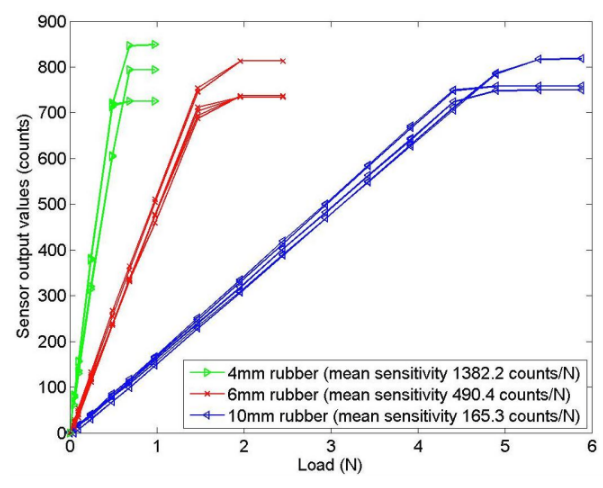
\includegraphics[width=0.5\textwidth]{figures/Load_vs_SensorvsThickness.png}
        \caption{Correlation between load and pressure readings at different thicknesses of polyurethane\cite{chuah2012composite}}
        \label{fig:my_label}
    \end{figure}

    The research done by the Contact Behavior of Soft Spherical Tactile Sensors\cite{youssefian2014contact} group demonstrated a similar method for calculating a pressure vector using magnets and hall effect sensors, despite the difference the math used to convert from readings to a pressure vector proved very useful to calculate out pressure vector using the 7 sensors on the foot of the robot. 
    \subsubsection{Communication Protocol}
   		\paragraph{Processor cycles}
   			The main purpose of the mothervboard is to receive data from teh computer over USB HID, parse, process and distribute to the motors accordingly. After speaking with Boston dynamics and deciding that for a reliable dynamics controller we would ideally have a control loop speed of \~ 1kHz at the highest level. This means that in 1 ms the micro controller must receive 64 bytes of data from the onboard computer, parse it to determine the type of command being sent to the motors, whether it is a position, velocity or torque setpoint, popuate the buffer and send through spi to each motor assuming all read and writes to memory and gpio is atomic, the time for data transfer can be calculated. \newline
     			
			\begin{gather*}
			\text{Clock Speed} = 384 \text{MHz}\\
   			\text{Data Size} = 16 \text{bits}\\
   			\text{SPI Transfer Speed} = 24 \frac{\text{Mbits}}{\text{s}}\\
   			\text{Size of SPI Package}= 5\\
   			\text{ No. Devices} = 5\\
   			\\
   			\\
   			\textbf{Time per clock cycle}\\
   			\frac{1}{\text{Clock Speed}}\\
   			\frac{1}{384000000}\\
   			 = 2.5*10^{-9} \tiny{\text{s}}\\
   			 \\
   			 \\
   			\textbf{No. bits per leg}\\
				\text{Data Size} * \text{Size of SPI Package} * \text{No. Devices}\\
				= 16 \tiny{\frac{\text{bits}}{\tiny{\text{packet}}}} * 5\frac{\text{packets}}{\text{device}} * 5\text{Devices} \\
				= 400 \tiny{\frac{\text{bits}}{\text{leg}}}\\
				\\
				\\
				\textbf{No. Clock cycles per SPI bit}\\
				\frac{\text{Clock Speed}}{\text{SPI	Transfer Speed}}\\
				\tiny{\frac{384\text{MHz}}{24\frac{\text{MHz}}{\text{s}}}}\\ 
				 =16\tiny{\text{Clock Cycles}}\\
			\\
			\\
			\textbf{Time to update a single leg}\\
			\text{No. Clock cycles per SPI bit} * \text{Time per clock cycle}\\
			16 * 2.5*10^{-9}\\
			=4*10^{-8}\text{s}\\
			\\
			\\
			\textbf{Time to update all legs}\\
			\text{Time to update a single leg} * \text{No. Legs}\\
			4*10^{-8}* 4\\
		    =1.6*10^{-7}\text{s}\\
			\end{gather*}  
			Using the same SPI channel and DMA, the total time to transfer all data to each of the legs would be \~ 1.6*10$^{-7}$s, this will allow the USB packet to be received, transmitted to the motors and the updated data returned to to the computer via an updated USB pacet. \newline
		
		Continuing with the assumption of atomic data transfers the use of separate SPI channels for each leg would allow for update speeds of 4*10$^{-8}$s minimizing the total time in between receiving and sending a return packet. This would be the optimal solution as it allows us to keep the 1ms round trip for usb to be keot as well as allowing for other processes to be run.  
		
        \paragraph{Micro-controller to Micro-controller}
        The decision on how to communicate between the master micro controller and the multiple salves through out the system came down to ease of re usability. The major communication options included ${I^2c}$, SPI, Can Bus, RS485 serial and RS232 Serial. The following is a table giving pros and cons of each choice.
    \begin{table}[H]
        \centering
        \begin{tabular}{|p{2cm}|p{6cm}|p{6cm}|}
    \hline
      Protocol   & Pros & Cons \\
    \hline
         \multirow{4}{*}{${I^2c}$} & Simple 2 wire interface & Requires independent addresses on each device \\
         & Easy Daisy chaining & Requires independent firmware to be flashed to each motor \\
         & Available on most micro controllers & Non synchronous \\
         & Supports DMA & Requires motor to be re flashed to move to a different location \\
         \hline
         \multirow{6}{*}{SPI} & Synchronous & Requires 4 wires to interface \\
         & Max baud rate of ~16.5 Mbaud &   \\
         & Supports DMA &  \\
         & Available on most microcontrollers & \\
         & Daisychainable & \\
         & Allows for multiple slaves to share one chip select line therefore no addressing & \\
         \hline
         \multirow{2}{*}{Can Bus} & Designed to be daisy chained  & Not available on most micro controllers \\
         & Simple 2 Wire interface & Slow  \\
         \hline
        \multirow{3}{*}{RS485 Serial}& Simple to use & Requires external IC\\
         &Designed to daisy chain & Slow \\
         & & Requires a software address be set\\
         \hline
         \multirow{3}{*}{RS232 Serial}& Available on most micro controllers & Slow\\
         & Simple to use & non synchronous \\
         & No hardware addresses needed & Difficult to daisy chain but possible\\
         
    \hline
    \end{tabular}
        \caption{Pros \& Cons of each communication protocol}
        \label{tab:my_label}
    \end{table}
   After researching in depth into each of these protocols taking into development time, limitation of resources such as space on circuit boards and ease of communication between micro controllers chosen, SPI was the final choice. The micro controllers used in the servo, foot pressure sensor and IMU breakout boards communicate back to the master micro controller through a daisy chained SPI DMA protocol where the packet of data is sent to the first object in the chain, the reply from the previous cycle is passed on as a return packet to the next, and so on until the final packet reaches the final micro controller and returns the packet of results to the main micro controller. The flow of data for an example leg is shown in the figure below.
   \begin{figure}[H]
       \centering
       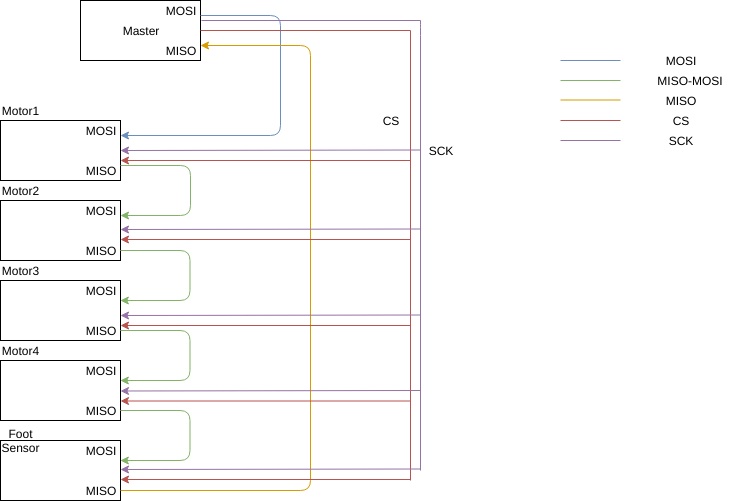
\includegraphics[width=0.6\textwidth]{figures/Leg_Flow_Dragram.png}
       \caption{Flow of data through a leg}
       \label{fig:my_label}
   \end{figure}
        \paragraph{Micro-controller to Computer}
        There were many fewer options for communicating between a computer and the master micro controller. The major solutions included Ethernet, USB HID and uart over USB. These options each have their advantages and disadvantages. Ethernet, this requires external supporting circuitry to interface between the micro controller and computer, this combined with the priority level of the networking stack on any Debian distribution of Linux including Ubuntu eliminated this option as a viable solution. Usart over USB was a viable option as the USB communication stack is marginally higher than the networking stack however usb to Usart is limited to \~2 Mbits/s. This meant that the throughput would not be enough for the robot to function reliably. USB HID communicates a 54 kbyte packet, reliably at 1ms. The HID USB stack is also the communication stack with the highest priority in any Debian based Linux system. therefore it is the least likely to lose a packet or have a data transmission error. 

\subsection{Software and Controls}

\subsubsection{Low-Level Control Software} 
The low level control software of the robot can be broken down into four distinct subcategories. These include the master controller, foot sensors, motors and IMUs. 
    \subsubsection{Master Controller}
    This controller receives trajectory points from the computer over USB HID, the controller then parses the data received to each motor. This controller performs calculations in order to optimize leg trajectory and paths. The data is packaged into four byte packets shown below.  
    \begin{figure}[H]
    \centering
    \begin{tabular}{|c|c|c|c|c|}
    \hline
     Device ID& Command & Val 1 & Val 2 & Val 3\\
    \hline
    \end{tabular}
    \caption{Data packet structure}
    \label{fig:my_label}
\end{figure}
The data is then sent to the motors, foot sensors and any other devices connected in the chain. Due to the nature of the system the data must be sent in order of the last device first as shown below. 
\begin{figure}[H]
    \centering
    \begin{tabular}{|c|c|c|c|c|}
    \hline
        Foot Sensor & Motor 4 & Motor 3 & Motor 2 & Motor 1  \\
        \hline
    \end{tabular}
    \caption{Order of packets sent to a leg}
    \label{fig:my_label}
\end{figure}
The path of data follows the structure below.

\begin{longtable}{|r|p{0.9\textwidth}|}
   \hline
   Packet & Action of data\\
   \hline
      {Packet 1} &  {\begin{itemize}
                    \item Motor 1 Receives the Foot Sensor packet, replies previous position, velocity and torque to motor 2
                    \item Motor 2 Receives return data from Motor 1 and replies its data to Motor 3
                    \item Motor 3 Receives return data from Motor 2 and replies its data to Motor 4 
                    \item Motor 4 Receives return data from Motor 3 and replies its data to the foot sensor 
                    \item The foot Sensor Receives return data from Motor 4 and replies the readings from the pressure sensors to the master controller
                 \end{itemize}}\\
                 \hline
      {Packet 2} &  {\begin{itemize}
                    \item Motor 1 Receives the Motor 4 packet, replies the Foot Sensor packet to motor 2
                    \item Motor 2 Receives the Foot Sensor packet and replies Motor 1 data to Motor 3
                    \item Motor 3 Receives return data from Motor 1 and replies Motor 2 data to Motor 4 
                    \item Motor 4 Receives return data from Motor 2 and replies Motor 3 data to the foot sensor 
                    \item The foot Sensor Receives return data from Motor 3 and replies Motor 4 data to the master controller
                 \end{itemize}}\\
                 \hline
      {Packet 3} &  {\begin{itemize}
                    \item Motor 1 Receives the Motor 3 packet, replies the Motor 4 packet to motor 2
                    \item Motor 2 Receives the Motor 4 packet and replies the Foot Sensor packet to Motor 3
                    \item Motor 3 Receives the Foot Sensor packet and replies Motor 1 data to Motor 4 
                    \item Motor 4 Receives return data from Motor 1 and replies Motor 2 data to the foot sensor 
                    \item The foot Sensor Receives return data from Motor 2 and replies Motor 3 data to the master controller
                 \end{itemize}}\\
                 \hline
     {Packet 4} &  {\begin{itemize}
                    \item Motor 1 Receives the Motor 2 packet, replies the Motor 3 packet to motor 2
                    \item Motor 2 Receives the Motor 3 packet and replies the Motor 4 packet to Motor 3
                    \item Motor 3 Receives the Motor 4 packet and replies Motor 1 data to Motor 4 
                    \item Motor 4 Receives the Foot Sensor packet and replies Motor 1 data to the foot sensor 
                    \item The foot Sensor Receives return data from Motor 1 and replies Motor 2 data to the master controller
                 \end{itemize}}\\
                 \hline
    {Packet 5} &  {\begin{itemize}
                    \item Motor 1 Receives the Motor 1 packet, replies the Motor 2 packet to motor 2
                    \item Motor 2 Receives the Motor 2 packet and replies the Motor 3 packet to Motor 3
                    \item Motor 3 Receives the Motor 3 packet and replies Motor 4 packet to Motor 4 
                    \item Motor 4 Receives the Foot Sensor packet and replies Motor 1 data to the foot sensor 
                    \item The foot Sensor receives Foot Sensor packet and replies Motor 1 data to the master controller
                 \end{itemize}}\\
    \hline
\end{longtable}

\noindent Once the cycle is completed the motors update the PID controllers, the foot sensors collect the pressure data and the cycle is looped. The return packet order is shown below.
\begin{figure}[H]
    \centering
    \begin{tabular}{|c|c|c|c|c|}
    \hline
        Motor 1 & Motor 2 & Motor 3 & Motor 4 & Foot Sensor \\
        \hline
    \end{tabular} 
    \caption{Order of Data returned from a leg}
    \label{fig:my_label}
\end{figure}

\subsubsection{Motors}
    When the motor receives a packet it checks if the first byte if the packet and compares it to the Dev ID of the motor. If the device Id does not match the first byte of the packet it is stages for transmission on the next packet received. If the packet is used to update that motor, the second byte of the packet is checked and compared to different known options. 
    \begin{table}[H]
        \centering
        \begin{tabular}{|c|c|}
        \hline
            Value & Command \\
            \hline
            0x22 & Update device ID based on byte 3 of the packet\\
            0x47 & Updates Position PID constants based on bytes 3,4,5 of the packet \\
            0x48 & Updates Velocity PID constants based on bytes 3,4,5 of the packet \\
            0x49 & Updates Torque PID constants based on bytes 3,4,5 of the packet \\
             0x91 & Updated position setpoint in Postion PID loop\\
            0x92 & Updated position setpoint in Velocity PID loop\\
            0x93 & Updated position setpoint in Torque PID loop\\
            \hline
            \end{tabular}
        \caption{Command values for servo}
        \label{tab:my_label}
    \end{table}
In between receiving packets the motors run multiple PID loops simultaneously to control position, torque and velocity at an ~161kHz refresh rate.
\subsubsection{IMU}
The IMU micro controller continuously samples the BNO055, recording the current gyroscope, acceleration and magnetometer data. On request from the master controller the IMU checks byte 1 and compares it to the device ID, if it matches it compares byte 2 to the list of known commands and replies accordingly which can be see below.
\begin{table}[H]
        \centering
        \begin{tabular}{|c|c|}
        \hline
            Value & Command \\
            \hline
            0x22 & Update device ID based on byte 3 of the packet\\
            0x37 & get gyroscope data\\
            0x38 & get accelerometer data\\
            0x39 & get magnetometer data\\
            \hline
            \end{tabular}
        \caption{Command values for IMU}
        \label{tab:my_label}
    \end{table}

\subsubsection{Foot Sensor}
Smurlarly to the IMU, the foot sensor micro controller continuously samples the 7 pressure sensors. On request from the master controller the foot sensor checks byte 1 and compares it to the device ID, if it matches it compares byte 2 to the list of known commands and replies accordingly which can be see below.
\begin{table}[H]
        \centering
        \begin{tabular}{|c|c|}
        \hline
            Value & Command \\
            \hline
            0x22 & Update device ID based on byte 3 of the packet\\
            0x32 & return most recent foot pressure sensor readings\\
            \hline
            \end{tabular}
        \caption{Command values for Foot sensor}
        \label{tab:my_label}
    \end{table}

\subsubsection{High-Level Control Software}
The High-Level Controllers’ jobs’ to run the kinematics and dynamics. This will include balancing, foot-step planning, and all the gaits we are planning on developing. The software written must have a few key objectives to hit to be considered useful for this application.  
\begin{enumerate}
    \item Real-time performance with a guaranteed response time of under 2ms
    \item Open-source and easily modifiable if needed
    \item Able to communicate quickly to our custom components and off-the-shelf components, like cameras, IMUs and other microcontrollers.
\end{enumerate}
With this in mind, there were a few options we found.

\subsubsection{Software Platforms}
\paragraph*{Bowler Studio}
Bowler Studio is a robot development application that combines scripting and device management with powerful control and processing features. It is comprised of two major parts: Bowler Studio, a development and visualization tool, and Bowler Kernel, a low-level platform designed to run at high cycle rates on Linux machines. The entire system is developed in Java, giving us developmental flexibility when it comes to operating systems, Linux distributions, or hardware platforms. It also improves development speed, since a library package manager like Gradle or Maven can be used. Previous versions of SmallKat were developed with Bowler due to its quick bring-up period. However, there are a few major shortcomings for Bowler Studio. The first is its adoption. Both Bowler Studio and Bowler Kernel are not widely used in the field of robotics. Using a platform like this will push its stability and performance to the max.
% Need to cite Bowler Studio in this paragraph
% TODO: Add more about Bowler Studio's Weaknesses and strengths
% TODO: Add a table with Bowler Studio's Weakness and strengths

\paragraph*{Robot Operating System (ROS)}
ROS, or Robot Operating System, is a widely used open-source robotics platform designed for adaptability and ease-of-bring-up for new robotic platforms. There are currently two major versions of ROS: ROS 1 and ROS 2.

ROS 1 has been tried and tested in the real world for over a decade. It is written in C and C++ and uses TCP/IP to communicate between processes, or nodes. ROS 1 is a really powerful tool for research and development, due to its adaptability and customizability. ROS's biggest advantage is the shear amount of packages developed for it. From camera software to SLAM algorithms to kinematics functions, ROS 1's community adoption along its open-source nature has led to a surplus of open-source packages that makes development easier. However, ROS 1 has 2 major downfalls: its speed and its security. Since ROS 1 is built using a networking back-end, the communication speeds between nodes is slow and unreliable. Testing proved that the guaranteed real-time performance for ROS 1 is about 100ms, over 100x slower than what we need for our system. It also relies on all ports to be open for good communication, making it a security nightmare. Most robotic solutions are initially developed in ROS for quick development time, but are then ported to a custom platform once key algorithms and functions are developed. Other research and development platforms, similar to ours, use ROS as a user interface and testing suite, with custom software written to communicate with ROS and the hardware.

ROS 2 is an attempt to fix the multitude of problems with ROS 1. It uses sockets instead of TCP/IP protocol for faster communication between nodes. It also implements new security protocols as a part of the platform. It is also built in a way where any language can be used, because its core is easily wrapped by any modern language. 
However, ROS 2 still has its issues. For starters, ROS 2 is relatively new: just 2 years old in stable form. It is not very feature-rich, and is not backwards compatible with ROS 1 packages (there is a backwards compatibility tool, but is very buggy at best). The second big problem is the instability of speed. ROS 2 boasts that it has been built to be real-time. However testing this claim, we found that although it could guarantee a 1ms loop 95\% of the time, the cycle time varied greatly - from 10 microseconds to 2.7 milliseconds.

\paragraph*{Custom Platform}
Since neither ROS 1/2 nor Bowler Studio is exactly what we were looking for, we considered writing a custom platform. The platform would be written in C and C++ and would likely communicate between processes using named pipes. This would allow for cross-platformability between Linux, Windows, and macOS, because every modern operating system has some implementation of named pipes. Communicating through named pipes is also extremely fast, because it is just reading and writing to files. The other communication method discussed was sockets. The main benefit is that they can be easily integrated for communication over Ethernet or WIFI. However, developing a custom platform is complicated and adds a lot of work and development time to ensure stability and functionality.

\subsubsection{High-Level Controller}
In the end, we decided to use Bowler Studio for the High-Level Controller. It offers cross-platformability and easy development due to its Java backbone. It also is relatively stable although not used much in the industry.

\subsubsection{Localization and User Control Software}
For the Localization and User Control Software, we decided on using ROS 1 due to its stability and wide range of open-source packages. The Localization and User Control Software will be split into two major sections: Visualization and Mapping, and User Control.

\paragraph*{Visualization and Mapping}
Visualization and Mapping will be utilizing the multitude of SLAM and navigation algorithms built into ROS 1. It takes in input from the on-board camera, and provides direction and velocity to the High-Level Controller. This allows us to easily implement a fully autonomous robot capable of exploring new areas.

\paragraph*{User Control}
The user control feature will have two parts: control and supervision. The control part will allow users to initiate gaits and control them remotely from another computer. It will also allow for initiating the autonomy function built in to SmallKat. The supervision portion will give the user the capability of watching different key variables, like joint angles, relative position, and body position relative to the world. This will help with debugging while developing on SmallKat.
\subsection{Mechanical Design}
    \subsubsection{Design Considerations}
            \begin{itemize} % I'm gonna make this a paragraph if i should even keep it here
            \item 
            \end{itemize}
     \subsubsection{Controls Equations}
     \begin{table}[H]
        \centering
        \begin{tabular}{|c|c|c|c|c|}
        \hline
            Link & a & $\alpha$ & d & $\theta$ \\
            \hline
            1 & 0 & $\theta_1$ + 90& 0& 0\\
            2 & $a_1$ & 0 & 0 &$\theta_2$ \\
            3 & $a_2$ & 0 & 0 &$\theta_3$ \\
            4 & $a_3$ & 0 & 0 &$\theta_4$ \\
            \hline
            \end{tabular}
        \caption{Table of DH parameters}
        \label{tab:my_label}
    \end{table}
    
    \begin{figure}[H]
    \centering
    \begin{gather*}
    X = a_3*sin(\theta_2+\theta_3)+a_2*sin(\theta2)+a_4*sin(\theta_2+\theta_3+\theta_4)\\
    Y = sin(\theta_1)*(a_1+a_3*cos(\theta_2+\theta_3)+a_2*cos(\theta_2)+a_4*cos(\theta_2+\theta_3+\theta_4))\\
    Z = -cos(\theta_1)*(a_1+a_3*cos(\theta_2+\theta_3)+a_2*cos(\theta_2)+a_4*cos(\theta_2+\theta_3+\theta_4))
    \end{gather*}
    
    \caption{Forward Positional Kinematics}
    \label{fig:my_label}
    \end{figure}
    
    \begin{figure}[H]
    \centering
    \begin{gather*}
    X = a_3*sin(\theta_2+\theta_3)+a_2*sin(\theta2)+a_4*sin(\theta_2+\theta_3+\theta_4)\\
    Y = sin(\theta_1)*(a_1+a_3*cos(\theta_2+\theta_3)+a_2*cos(\theta_2)+a_4*cos(\theta_2+\theta_3+\theta_4))\\
    Z = -cos(\theta_1)*(a_1+a_3*cos(\theta_2+\theta_3)+a_2*cos(\theta_2)+a_4*cos(\theta_2+\theta_3+\theta_4))
    \end{gather*}
    
    \caption{Forward torque Kinematics}
    \label{fig:my_label}
    \end{figure}

     \subsubsection{4 dof}
     \subsubsection{Motor Tests}